\documentclass[1p]{elsarticle_modified}
%\bibliographystyle{elsarticle-num}

%\usepackage[colorlinks]{hyperref}
%\usepackage{abbrmath_seonhwa} %\Abb, \Ascr, \Acal ,\Abf, \Afrak
\usepackage{amsfonts}
\usepackage{amssymb}
\usepackage{amsmath}
\usepackage{amsthm}
\usepackage{scalefnt}
\usepackage{amsbsy}
\usepackage{kotex}
\usepackage{caption}
\usepackage{subfig}
\usepackage{color}
\usepackage{graphicx}
\usepackage{xcolor} %% white, black, red, green, blue, cyan, magenta, yellow
\usepackage{float}
\usepackage{setspace}
\usepackage{hyperref}

\usepackage{tikz}
\usetikzlibrary{arrows}

\usepackage{multirow}
\usepackage{array} % fixed length table
\usepackage{hhline}

%%%%%%%%%%%%%%%%%%%%%
\makeatletter
\renewcommand*\env@matrix[1][\arraystretch]{%
	\edef\arraystretch{#1}%
	\hskip -\arraycolsep
	\let\@ifnextchar\new@ifnextchar
	\array{*\c@MaxMatrixCols c}}
\makeatother %https://tex.stackexchange.com/questions/14071/how-can-i-increase-the-line-spacing-in-a-matrix
%%%%%%%%%%%%%%%

\usepackage[normalem]{ulem}

\newcommand{\msout}[1]{\ifmmode\text{\sout{\ensuremath{#1}}}\else\sout{#1}\fi}
%SOURCE: \msout is \stkout macro in https://tex.stackexchange.com/questions/20609/strikeout-in-math-mode

\newcommand{\cancel}[1]{
	\ifmmode
	{\color{red}\msout{#1}}
	\else
	{\color{red}\sout{#1}}
	\fi
}

\newcommand{\add}[1]{
	{\color{blue}\uwave{#1}}
}

\newcommand{\replace}[2]{
	\ifmmode
	{\color{red}\msout{#1}}{\color{blue}\uwave{#2}}
	\else
	{\color{red}\sout{#1}}{\color{blue}\uwave{#2}}
	\fi
}

\newcommand{\Sol}{\mathcal{S}} %segment
\newcommand{\D}{D} %diagram
\newcommand{\A}{\mathcal{A}} %arc


%%%%%%%%%%%%%%%%%%%%%%%%%%%%%5 test

\def\sl{\operatorname{\textup{SL}}(2,\Cbb)}
\def\psl{\operatorname{\textup{PSL}}(2,\Cbb)}
\def\quan{\mkern 1mu \triangleright \mkern 1mu}

\theoremstyle{definition}
\newtheorem{thm}{Theorem}[section]
\newtheorem{prop}[thm]{Proposition}
\newtheorem{lem}[thm]{Lemma}
\newtheorem{ques}[thm]{Question}
\newtheorem{cor}[thm]{Corollary}
\newtheorem{defn}[thm]{Definition}
\newtheorem{exam}[thm]{Example}
\newtheorem{rmk}[thm]{Remark}
\newtheorem{alg}[thm]{Algorithm}

\newcommand{\I}{\sqrt{-1}}
\begin{document}

%\begin{frontmatter}
%
%\title{Boundary parabolic representations of knots up to 8 crossings}
%
%%% Group authors per affiliation:
%\author{Yunhi Cho} 
%\address{Department of Mathematics, University of Seoul, Seoul, Korea}
%\ead{yhcho@uos.ac.kr}
%
%
%\author{Seonhwa Kim} %\fnref{s_kim}}
%\address{Center for Geometry and Physics, Institute for Basic Science, Pohang, 37673, Korea}
%\ead{ryeona17@ibs.re.kr}
%
%\author{Hyuk Kim}
%\address{Department of Mathematical Sciences, Seoul National University, Seoul 08826, Korea}
%\ead{hyukkim@snu.ac.kr}
%
%\author{Seokbeom Yoon}
%\address{Department of Mathematical Sciences, Seoul National University, Seoul, 08826,  Korea}
%\ead{sbyoon15@snu.ac.kr}
%
%\begin{abstract}
%We find all boundary parabolic representation of knots up to 8 crossings.
%
%\end{abstract}
%\begin{keyword}
%    \MSC[2010] 57M25 
%\end{keyword}
%
%\end{frontmatter}

%\linenumbers
%\tableofcontents
%
\newcommand\colored[1]{\textcolor{white}{\rule[-0.35ex]{0.8em}{1.4ex}}\kern-0.8em\color{red} #1}%
%\newcommand\colored[1]{\textcolor{white}{ #1}\kern-2.17ex	\textcolor{white}{ #1}\kern-1.81ex	\textcolor{white}{ #1}\kern-2.15ex\color{red}#1	}

{\Large $\underline{12n_{0759}~(K12n_{0759})}$}

\setlength{\tabcolsep}{10pt}
\renewcommand{\arraystretch}{1.6}
\vspace{1cm}\begin{tabular}{m{100pt}>{\centering\arraybackslash}m{274pt}}
\multirow{5}{120pt}{
	\centering
	\includegraphics[width=112pt]{../../../GIT/diagram.site/Diagrams/png/2848_12n_0759.png}\\
\ \ \ A knot diagram\footnotemark}&
\allowdisplaybreaks
\textbf{Linearized knot diagam} \\
\cline{2-2}
 &
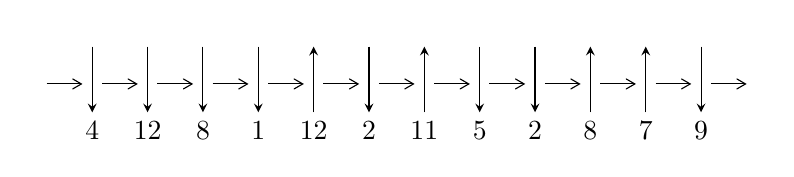
\begin{tikzpicture}[x=20pt, y=17pt]
	% nodes
	\node (C0) at (0, 0) {};
	\node (C1) at (1, 0) {};
	\node (C1U) at (1, +1) {};
	\node (C1D) at (1, -1) {4};

	\node (C2) at (2, 0) {};
	\node (C2U) at (2, +1) {};
	\node (C2D) at (2, -1) {12};

	\node (C3) at (3, 0) {};
	\node (C3U) at (3, +1) {};
	\node (C3D) at (3, -1) {8};

	\node (C4) at (4, 0) {};
	\node (C4U) at (4, +1) {};
	\node (C4D) at (4, -1) {1};

	\node (C5) at (5, 0) {};
	\node (C5U) at (5, +1) {};
	\node (C5D) at (5, -1) {12};

	\node (C6) at (6, 0) {};
	\node (C6U) at (6, +1) {};
	\node (C6D) at (6, -1) {2};

	\node (C7) at (7, 0) {};
	\node (C7U) at (7, +1) {};
	\node (C7D) at (7, -1) {11};

	\node (C8) at (8, 0) {};
	\node (C8U) at (8, +1) {};
	\node (C8D) at (8, -1) {5};

	\node (C9) at (9, 0) {};
	\node (C9U) at (9, +1) {};
	\node (C9D) at (9, -1) {2};

	\node (C10) at (10, 0) {};
	\node (C10U) at (10, +1) {};
	\node (C10D) at (10, -1) {8};

	\node (C11) at (11, 0) {};
	\node (C11U) at (11, +1) {};
	\node (C11D) at (11, -1) {7};

	\node (C12) at (12, 0) {};
	\node (C12U) at (12, +1) {};
	\node (C12D) at (12, -1) {9};
	\node (C13) at (13, 0) {};

	% arrows
	\draw[->,>={angle 60}]
	(C0) edge (C1) (C1) edge (C2) (C2) edge (C3) (C3) edge (C4) (C4) edge (C5) (C5) edge (C6) (C6) edge (C7) (C7) edge (C8) (C8) edge (C9) (C9) edge (C10) (C10) edge (C11) (C11) edge (C12) (C12) edge (C13) ;	\draw[->,>=stealth]
	(C1U) edge (C1D) (C2U) edge (C2D) (C3U) edge (C3D) (C4U) edge (C4D) (C5D) edge (C5U) (C6U) edge (C6D) (C7D) edge (C7U) (C8U) edge (C8D) (C9U) edge (C9D) (C10D) edge (C10U) (C11D) edge (C11U) (C12U) edge (C12D) ;
	\end{tikzpicture} \\
\hhline{~~} \\& 
\textbf{Solving Sequence} \\ \cline{2-2} 
 &
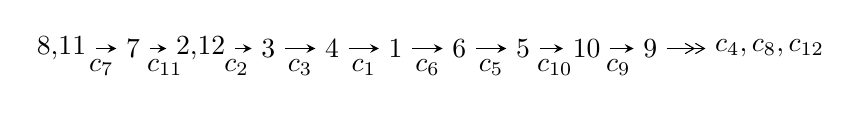
\begin{tikzpicture}[x=23pt, y=7pt]
	% node
	\node (A0) at (-1/8, 0) {8,11};
	\node (A1) at (1, 0) {7};
	\node (A2) at (33/16, 0) {2,12};
	\node (A3) at (25/8, 0) {3};
	\node (A4) at (33/8, 0) {4};
	\node (A5) at (41/8, 0) {1};
	\node (A6) at (49/8, 0) {6};
	\node (A7) at (57/8, 0) {5};
	\node (A8) at (65/8, 0) {10};
	\node (A9) at (73/8, 0) {9};
	\node (C1) at (1/2, -1) {$c_{7}$};
	\node (C2) at (3/2, -1) {$c_{11}$};
	\node (C3) at (21/8, -1) {$c_{2}$};
	\node (C4) at (29/8, -1) {$c_{3}$};
	\node (C5) at (37/8, -1) {$c_{1}$};
	\node (C6) at (45/8, -1) {$c_{6}$};
	\node (C7) at (53/8, -1) {$c_{5}$};
	\node (C8) at (61/8, -1) {$c_{10}$};
	\node (C9) at (69/8, -1) {$c_{9}$};
	\node (A10) at (11, 0) {$c_{4},c_{8},c_{12}$};

	% edge
	\draw[->,>=stealth]	
	(A0) edge (A1) (A1) edge (A2) (A2) edge (A3) (A3) edge (A4) (A4) edge (A5) (A5) edge (A6) (A6) edge (A7) (A7) edge (A8) (A8) edge (A9) ;
	\draw[->>,>={angle 60}]	
	(A9) edge (A10);
\end{tikzpicture} \\ 

\end{tabular} \\

\footnotetext{
The image of knot diagram is generated by the software ``\textbf{Draw programme}" developed by Andrew Bartholomew(\url{http://www.layer8.co.uk/maths/draw/index.htm\#Running-draw}), where we modified some parts for our purpose(\url{https://github.com/CATsTAILs/LinksPainter}).
}\phantom \\ \newline 
\centering \textbf{Ideals for irreducible components\footnotemark of $X_{\text{par}}$} 
 
\begin{align*}
I^u_{1}&=\langle 
471524796 u^{36}-5108104574 u^{35}+\cdots+1495255511 b+27229387303,\\
\phantom{I^u_{1}}&\phantom{= \langle  }12296434297 u^{36}-69707922846 u^{35}+\cdots+14952555110 a-105681891942,\\
\phantom{I^u_{1}}&\phantom{= \langle  }u^{37}-8 u^{36}+\cdots+54 u-10\rangle \\
I^u_{2}&=\langle 
- u^{17} a- u^{17}+\cdots+b+a,\;u^{16} a+2 u^{17}+\cdots+a+5,\;u^{18}+5 u^{17}+\cdots+3 u-1\rangle \\
I^u_{3}&=\langle 
u^{16}+5 u^{15}+\cdots+b+3,\;-3 u^{17}-17 u^{16}+\cdots+2 a-11,\;u^{18}+5 u^{17}+\cdots+13 u+2\rangle \\
\\
\end{align*}
\raggedright * 3 irreducible components of $\dim_{\mathbb{C}}=0$, with total 91 representations.\\
\footnotetext{All coefficients of polynomials are rational numbers. But the coefficients are sometimes approximated in decimal forms when there is not enough margin.}
\newpage
\renewcommand{\arraystretch}{1}
\centering \section*{I. $I^u_{1}= \langle 4.72\times10^{8} u^{36}-5.11\times10^{9} u^{35}+\cdots+1.50\times10^{9} b+2.72\times10^{10},\;1.23\times10^{10} u^{36}-6.97\times10^{10} u^{35}+\cdots+1.50\times10^{10} a-1.06\times10^{11},\;u^{37}-8 u^{36}+\cdots+54 u-10 \rangle$}
\flushleft \textbf{(i) Arc colorings}\\
\begin{tabular}{m{7pt} m{180pt} m{7pt} m{180pt} }
\flushright $a_{8}=$&$\begin{pmatrix}1\\0\end{pmatrix}$ \\
\flushright $a_{11}=$&$\begin{pmatrix}0\\u\end{pmatrix}$ \\
\flushright $a_{7}=$&$\begin{pmatrix}1\\u^2\end{pmatrix}$ \\
\flushright $a_{2}=$&$\begin{pmatrix}-0.822363 u^{36}+4.66194 u^{35}+\cdots-40.6849 u+7.06781\\-0.315347 u^{36}+3.41621 u^{35}+\cdots+84.0045 u-18.2105\end{pmatrix}$ \\
\flushright $a_{12}=$&$\begin{pmatrix}u\\u^3+u\end{pmatrix}$ \\
\flushright $a_{3}=$&$\begin{pmatrix}1.82105 u^{36}-14.2531 u^{35}+\cdots-80.8722 u+14.3323\\1.02354 u^{36}-7.91667 u^{35}+\cdots-50.2937 u+11.3771\end{pmatrix}$ \\
\flushright $a_{4}=$&$\begin{pmatrix}0.797516 u^{36}-6.33640 u^{35}+\cdots-30.5786 u+2.95520\\1.02354 u^{36}-7.91667 u^{35}+\cdots-50.2937 u+11.3771\end{pmatrix}$ \\
\flushright $a_{1}=$&$\begin{pmatrix}1.17552 u^{36}-8.86307 u^{35}+\cdots-58.6629 u+12.1412\\0.968604 u^{36}-9.68456 u^{35}+\cdots-102.310 u+21.5655\end{pmatrix}$ \\
\flushright $a_{6}=$&$\begin{pmatrix}4.28726 u^{36}-34.0282 u^{35}+\cdots-123.485 u+23.2929\\-2.54465 u^{36}+18.9069 u^{35}+\cdots+0.613399 u+3.92450\end{pmatrix}$ \\
\flushright $a_{5}=$&$\begin{pmatrix}-0.392450 u^{36}+5.68425 u^{35}+\cdots+113.422 u-20.8057\\1.18047 u^{36}-6.84211 u^{35}+\cdots+67.8836 u-17.4261\end{pmatrix}$ \\
\flushright $a_{10}=$&$\begin{pmatrix}- u\\u\end{pmatrix}$ \\
\flushright $a_{9}=$&$\begin{pmatrix}2.92308 u^{36}-21.9635 u^{35}+\cdots-55.9879 u+8.79131\\-2.66058 u^{36}+17.9266 u^{35}+\cdots+21.3706 u-3.21429\end{pmatrix}$\\&\end{tabular}
\flushleft \textbf{(ii) Obstruction class $= -1$}\\~\\
\flushleft \textbf{(iii) Cusp Shapes $= -\frac{12741675491}{1495255511} u^{36}+\frac{101934190202}{1495255511} u^{35}+\cdots+\frac{510036125358}{1495255511} u-\frac{91985646542}{1495255511}$}\\~\\
\newpage\renewcommand{\arraystretch}{1}
\flushleft \textbf{(iv) u-Polynomials at the component}\newline \\
\begin{tabular}{m{50pt}|m{274pt}}
Crossings & \hspace{64pt}u-Polynomials at each crossing \\
\hline $$\begin{aligned}c_{1},c_{4}\end{aligned}$$&$\begin{aligned}
&u^{37}-11 u^{36}+\cdots-158 u+10
\end{aligned}$\\
\hline $$\begin{aligned}c_{2},c_{6}\end{aligned}$$&$\begin{aligned}
&u^{37}+20 u^{35}+\cdots+4 u+1
\end{aligned}$\\
\hline $$\begin{aligned}c_{3},c_{9}\end{aligned}$$&$\begin{aligned}
&u^{37}- u^{36}+\cdots+286 u+121
\end{aligned}$\\
\hline $$\begin{aligned}c_{5}\end{aligned}$$&$\begin{aligned}
&u^{37}-32 u^{36}+\cdots-3538944 u+262144
\end{aligned}$\\
\hline $$\begin{aligned}c_{7},c_{10},c_{11}\end{aligned}$$&$\begin{aligned}
&u^{37}+8 u^{36}+\cdots+54 u+10
\end{aligned}$\\
\hline $$\begin{aligned}c_{8},c_{12}\end{aligned}$$&$\begin{aligned}
&u^{37}+u^{36}+\cdots+5 u+1
\end{aligned}$\\
\hline
\end{tabular}\\~\\
\newpage\renewcommand{\arraystretch}{1}
\flushleft \textbf{(v) Riley Polynomials at the component}\newline \\
\begin{tabular}{m{50pt}|m{274pt}}
Crossings & \hspace{64pt}Riley Polynomials at each crossing \\
\hline $$\begin{aligned}c_{1},c_{4}\end{aligned}$$&$\begin{aligned}
&y^{37}+23 y^{36}+\cdots+1464 y-100
\end{aligned}$\\
\hline $$\begin{aligned}c_{2},c_{6}\end{aligned}$$&$\begin{aligned}
&y^{37}+40 y^{36}+\cdots-24 y-1
\end{aligned}$\\
\hline $$\begin{aligned}c_{3},c_{9}\end{aligned}$$&$\begin{aligned}
&y^{37}+19 y^{36}+\cdots-31218 y-14641
\end{aligned}$\\
\hline $$\begin{aligned}c_{5}\end{aligned}$$&$\begin{aligned}
&y^{37}-6 y^{36}+\cdots+51539607552 y-68719476736
\end{aligned}$\\
\hline $$\begin{aligned}c_{7},c_{10},c_{11}\end{aligned}$$&$\begin{aligned}
&y^{37}+32 y^{36}+\cdots+1176 y-100
\end{aligned}$\\
\hline $$\begin{aligned}c_{8},c_{12}\end{aligned}$$&$\begin{aligned}
&y^{37}+21 y^{36}+\cdots+y-1
\end{aligned}$\\
\hline
\end{tabular}\\~\\
\newpage\flushleft \textbf{(vi) Complex Volumes and Cusp Shapes}
$$\begin{array}{c|c|c}  
\text{Solutions to }I^u_{1}& \I (\text{vol} + \sqrt{-1}CS) & \text{Cusp shape}\\
 \hline 
\begin{aligned}
u &= -0.139810 + 0.947636 I \\
a &= \phantom{-}1.72762 - 0.66054 I \\
b &= -1.14617 - 0.94052 I\end{aligned}
 & \phantom{-}2.14502 - 0.46485 I & -1.94282 - 0.92392 I \\ \hline\begin{aligned}
u &= -0.139810 - 0.947636 I \\
a &= \phantom{-}1.72762 + 0.66054 I \\
b &= -1.14617 + 0.94052 I\end{aligned}
 & \phantom{-}2.14502 + 0.46485 I & -1.94282 + 0.92392 I \\ \hline\begin{aligned}
u &= \phantom{-}1.039010 + 0.115439 I \\
a &= -0.192987 + 0.037881 I \\
b &= -0.62037 + 1.63193 I\end{aligned}
 & \phantom{-}10.1014 + 11.1664 I & \phantom{-0.000000 } 0. - 6.23795 I \\ \hline\begin{aligned}
u &= \phantom{-}1.039010 - 0.115439 I \\
a &= -0.192987 - 0.037881 I \\
b &= -0.62037 - 1.63193 I\end{aligned}
 & \phantom{-}10.1014 - 11.1664 I & \phantom{-0.000000 -}0. + 6.23795 I \\ \hline\begin{aligned}
u &= \phantom{-}0.916293 + 0.067951 I \\
a &= \phantom{-}0.097764 + 0.172517 I \\
b &= \phantom{-}0.46237 - 1.48507 I\end{aligned}
 & \phantom{-}5.40488 + 5.68156 I & -1.59495 - 5.13236 I \\ \hline\begin{aligned}
u &= \phantom{-}0.916293 - 0.067951 I \\
a &= \phantom{-}0.097764 - 0.172517 I \\
b &= \phantom{-}0.46237 + 1.48507 I\end{aligned}
 & \phantom{-}5.40488 - 5.68156 I & -1.59495 + 5.13236 I \\ \hline\begin{aligned}
u &= \phantom{-}0.885871 + 0.114565 I \\
a &= \phantom{-}0.281357 + 0.113956 I \\
b &= -0.25335 - 1.47096 I\end{aligned}
 & \phantom{-}9.31086 + 0.52432 I & \phantom{-}3.94650 - 0.50356 I \\ \hline\begin{aligned}
u &= \phantom{-}0.885871 - 0.114565 I \\
a &= \phantom{-}0.281357 - 0.113956 I \\
b &= -0.25335 + 1.47096 I\end{aligned}
 & \phantom{-}9.31086 - 0.52432 I & \phantom{-}3.94650 + 0.50356 I \\ \hline\begin{aligned}
u &= \phantom{-}0.056118 + 1.111250 I \\
a &= -1.50526 + 0.77231 I \\
b &= \phantom{-}1.324570 + 0.077249 I\end{aligned}
 & \phantom{-}0.897651 + 0.070840 I & -4.00000 + 0. I\phantom{ +0.000000I} \\ \hline\begin{aligned}
u &= \phantom{-}0.056118 - 1.111250 I \\
a &= -1.50526 - 0.77231 I \\
b &= \phantom{-}1.324570 - 0.077249 I\end{aligned}
 & \phantom{-}0.897651 - 0.070840 I & -4.00000 + 0. I\phantom{ +0.000000I}\\
 \hline 
 \end{array}$$\newpage$$\begin{array}{c|c|c}  
\text{Solutions to }I^u_{1}& \I (\text{vol} + \sqrt{-1}CS) & \text{Cusp shape}\\
 \hline 
\begin{aligned}
u &= -0.609754 + 0.620108 I \\
a &= \phantom{-}0.782999 + 0.288087 I \\
b &= \phantom{-}0.627363 - 0.626705 I\end{aligned}
 & \phantom{-}2.48681 - 2.57040 I & -2.36259 + 3.28826 I \\ \hline\begin{aligned}
u &= -0.609754 - 0.620108 I \\
a &= \phantom{-}0.782999 - 0.288087 I \\
b &= \phantom{-}0.627363 + 0.626705 I\end{aligned}
 & \phantom{-}2.48681 + 2.57040 I & -2.36259 - 3.28826 I \\ \hline\begin{aligned}
u &= \phantom{-}0.086875 + 1.167150 I \\
a &= \phantom{-}1.63975 + 0.44424 I \\
b &= -1.11741 - 0.88125 I\end{aligned}
 & -4.39474 + 1.30377 I & -15.9395 + 0. I\phantom{ +0.000000I} \\ \hline\begin{aligned}
u &= \phantom{-}0.086875 - 1.167150 I \\
a &= \phantom{-}1.63975 - 0.44424 I \\
b &= -1.11741 + 0.88125 I\end{aligned}
 & -4.39474 - 1.30377 I & -15.9395 + 0. I\phantom{ +0.000000I} \\ \hline\begin{aligned}
u &= -0.245173 + 1.209770 I \\
a &= -0.978004 - 0.158481 I \\
b &= \phantom{-}0.640982 + 1.102120 I\end{aligned}
 & -0.79010 - 3.56350 I & \phantom{-0.000000 } 0 \\ \hline\begin{aligned}
u &= -0.245173 - 1.209770 I \\
a &= -0.978004 + 0.158481 I \\
b &= \phantom{-}0.640982 - 1.102120 I\end{aligned}
 & -0.79010 + 3.56350 I & \phantom{-0.000000 } 0 \\ \hline\begin{aligned}
u &= \phantom{-}0.443655 + 1.201050 I \\
a &= -1.79320 + 0.50024 I \\
b &= \phantom{-}0.819804 - 0.963504 I\end{aligned}
 & \phantom{-}5.97221 + 4.23436 I & \phantom{-0.000000 } 0 \\ \hline\begin{aligned}
u &= \phantom{-}0.443655 - 1.201050 I \\
a &= -1.79320 - 0.50024 I \\
b &= \phantom{-}0.819804 + 0.963504 I\end{aligned}
 & \phantom{-}5.97221 - 4.23436 I & \phantom{-0.000000 } 0 \\ \hline\begin{aligned}
u &= \phantom{-}0.435560 + 1.215640 I \\
a &= -1.06951 + 0.99559 I \\
b &= \phantom{-}0.263581 - 1.008440 I\end{aligned}
 & \phantom{-}1.85513 - 0.84698 I & \phantom{-0.000000 } 0 \\ \hline\begin{aligned}
u &= \phantom{-}0.435560 - 1.215640 I \\
a &= -1.06951 - 0.99559 I \\
b &= \phantom{-}0.263581 + 1.008440 I\end{aligned}
 & \phantom{-}1.85513 + 0.84698 I & \phantom{-0.000000 } 0\\
 \hline 
 \end{array}$$\newpage$$\begin{array}{c|c|c}  
\text{Solutions to }I^u_{1}& \I (\text{vol} + \sqrt{-1}CS) & \text{Cusp shape}\\
 \hline 
\begin{aligned}
u &= -0.295335 + 0.570556 I \\
a &= -0.576122 + 0.317004 I \\
b &= \phantom{-}0.130785 + 0.394729 I\end{aligned}
 & -0.109537 - 1.239830 I & -1.37448 + 5.92241 I \\ \hline\begin{aligned}
u &= -0.295335 - 0.570556 I \\
a &= -0.576122 - 0.317004 I \\
b &= \phantom{-}0.130785 - 0.394729 I\end{aligned}
 & -0.109537 + 1.239830 I & -1.37448 - 5.92241 I \\ \hline\begin{aligned}
u &= \phantom{-}0.614437 + 1.236310 I \\
a &= \phantom{-}0.902398 - 0.941361 I \\
b &= \phantom{-}0.392590 + 1.064250 I\end{aligned}
 & \phantom{-}6.68893 - 5.37975 I & \phantom{-0.000000 } 0 \\ \hline\begin{aligned}
u &= \phantom{-}0.614437 - 1.236310 I \\
a &= \phantom{-}0.902398 + 0.941361 I \\
b &= \phantom{-}0.392590 - 1.064250 I\end{aligned}
 & \phantom{-}6.68893 + 5.37975 I & \phantom{-0.000000 } 0 \\ \hline\begin{aligned}
u &= \phantom{-}0.434151 + 1.339220 I \\
a &= \phantom{-}1.76152 - 0.74711 I \\
b &= -1.14193 + 1.58433 I\end{aligned}
 & \phantom{-}1.00539 + 10.52360 I & \phantom{-0.000000 } 0 \\ \hline\begin{aligned}
u &= \phantom{-}0.434151 - 1.339220 I \\
a &= \phantom{-}1.76152 + 0.74711 I \\
b &= -1.14193 - 1.58433 I\end{aligned}
 & \phantom{-}1.00539 - 10.52360 I & \phantom{-0.000000 } 0 \\ \hline\begin{aligned}
u &= \phantom{-}0.38979 + 1.37969 I \\
a &= \phantom{-}0.93958 - 1.24376 I \\
b &= -0.37436 + 1.70929 I\end{aligned}
 & \phantom{-}4.58667 + 5.11314 I & \phantom{-0.000000 } 0 \\ \hline\begin{aligned}
u &= \phantom{-}0.38979 - 1.37969 I \\
a &= \phantom{-}0.93958 + 1.24376 I \\
b &= -0.37436 - 1.70929 I\end{aligned}
 & \phantom{-}4.58667 - 5.11314 I & \phantom{-0.000000 } 0 \\ \hline\begin{aligned}
u &= \phantom{-}0.48491 + 1.39397 I \\
a &= -1.66833 + 0.76934 I \\
b &= \phantom{-}1.01582 - 1.92652 I\end{aligned}
 & \phantom{-}5.3737 + 16.5878 I & \phantom{-0.000000 } 0 \\ \hline\begin{aligned}
u &= \phantom{-}0.48491 - 1.39397 I \\
a &= -1.66833 - 0.76934 I \\
b &= \phantom{-}1.01582 + 1.92652 I\end{aligned}
 & \phantom{-}5.3737 - 16.5878 I & \phantom{-0.000000 } 0\\
 \hline 
 \end{array}$$\newpage$$\begin{array}{c|c|c}  
\text{Solutions to }I^u_{1}& \I (\text{vol} + \sqrt{-1}CS) & \text{Cusp shape}\\
 \hline 
\begin{aligned}
u &= -0.456996 + 0.144661 I \\
a &= -0.60975 - 1.37109 I \\
b &= -0.583726 - 0.575126 I\end{aligned}
 & \phantom{-}3.13815 - 0.83302 I & -1.02036 + 3.40722 I \\ \hline\begin{aligned}
u &= -0.456996 - 0.144661 I \\
a &= -0.60975 + 1.37109 I \\
b &= -0.583726 + 0.575126 I\end{aligned}
 & \phantom{-}3.13815 + 0.83302 I & -1.02036 - 3.40722 I \\ \hline\begin{aligned}
u &= -0.05084 + 1.54951 I \\
a &= \phantom{-}0.027721 + 0.450422 I \\
b &= \phantom{-}0.223004 - 0.781521 I\end{aligned}
 & -7.37098 - 2.21708 I & \phantom{-0.000000 } 0 \\ \hline\begin{aligned}
u &= -0.05084 - 1.54951 I \\
a &= \phantom{-}0.027721 - 0.450422 I \\
b &= \phantom{-}0.223004 + 0.781521 I\end{aligned}
 & -7.37098 + 2.21708 I & \phantom{-0.000000 } 0 \\ \hline\begin{aligned}
u &= -0.12383 + 1.62650 I \\
a &= \phantom{-}0.376630 - 0.307169 I \\
b &= -0.973816 + 0.280615 I\end{aligned}
 & -5.40481 - 5.27286 I & \phantom{-0.000000 } 0 \\ \hline\begin{aligned}
u &= -0.12383 - 1.62650 I \\
a &= \phantom{-}0.376630 + 0.307169 I \\
b &= -0.973816 - 0.280615 I\end{aligned}
 & -5.40481 + 5.27286 I & \phantom{-0.000000 } 0 \\ \hline\begin{aligned}
u &= \phantom{-}0.270127\phantom{ +0.000000I} \\
a &= -2.08837\phantom{ +0.000000I} \\
b &= \phantom{-}0.620523\phantom{ +0.000000I}\end{aligned}
 & -1.19161\phantom{ +0.000000I} & -2.79840\phantom{ +0.000000I}\\
 \hline 
 \end{array}$$\newpage\newpage\renewcommand{\arraystretch}{1}
\centering \section*{II. $I^u_{2}= \langle - u^{17} a- u^{17}+\cdots+b+a,\;u^{16} a+2 u^{17}+\cdots+a+5,\;u^{18}+5 u^{17}+\cdots+3 u-1 \rangle$}
\flushleft \textbf{(i) Arc colorings}\\
\begin{tabular}{m{7pt} m{180pt} m{7pt} m{180pt} }
\flushright $a_{8}=$&$\begin{pmatrix}1\\0\end{pmatrix}$ \\
\flushright $a_{11}=$&$\begin{pmatrix}0\\u\end{pmatrix}$ \\
\flushright $a_{7}=$&$\begin{pmatrix}1\\u^2\end{pmatrix}$ \\
\flushright $a_{2}=$&$\begin{pmatrix}a\\u^{17} a+u^{17}+\cdots- a+2 u\end{pmatrix}$ \\
\flushright $a_{12}=$&$\begin{pmatrix}u\\u^3+u\end{pmatrix}$ \\
\flushright $a_{3}=$&$\begin{pmatrix}- u^{17} a-4 u^{16} a+\cdots+2 a- u\\- u^{17} a-4 u^{16} a+\cdots+a+1\end{pmatrix}$ \\
\flushright $a_{4}=$&$\begin{pmatrix}u^{16}+4 u^{15}+\cdots+a-1\\- u^{17} a-4 u^{16} a+\cdots+a+1\end{pmatrix}$ \\
\flushright $a_{1}=$&$\begin{pmatrix}- u^{16}-4 u^{15}+\cdots+a+2\\u^{17} a+4 u^{16} a+\cdots- a-1\end{pmatrix}$ \\
\flushright $a_{6}=$&$\begin{pmatrix}u^{15} a- u^{16}+\cdots- a+3\\u^{17} a+4 u^{16} a+\cdots- a-1\end{pmatrix}$ \\
\flushright $a_{5}=$&$\begin{pmatrix}u^{15} a- u^{16}+\cdots- a+3\\u^{17} a+4 u^{16} a+\cdots- a-1\end{pmatrix}$ \\
\flushright $a_{10}=$&$\begin{pmatrix}- u\\u\end{pmatrix}$ \\
\flushright $a_{9}=$&$\begin{pmatrix}- u^{16}-6 u^{15}+\cdots- a-2\\u^{17} a+4 u^{16} a+\cdots- a-1\end{pmatrix}$\\&\end{tabular}
\flushleft \textbf{(ii) Obstruction class $= -1$}\\~\\
\flushleft \textbf{(iii) Cusp Shapes $= 4 u^{16}+20 u^{15}+72 u^{14}+180 u^{13}+356 u^{12}+572 u^{11}+744 u^{10}+808 u^9+692 u^8+460 u^7+204 u^6+12 u^5-36 u^4-32 u^3+8 u^2+20 u-6$}\\~\\
\newpage\renewcommand{\arraystretch}{1}
\flushleft \textbf{(iv) u-Polynomials at the component}\newline \\
\begin{tabular}{m{50pt}|m{274pt}}
Crossings & \hspace{64pt}u-Polynomials at each crossing \\
\hline $$\begin{aligned}c_{1},c_{4}\end{aligned}$$&$\begin{aligned}
&(u^{18}+5 u^{17}+\cdots+3 u-1)^{2}
\end{aligned}$\\
\hline $$\begin{aligned}c_{2},c_{6}\end{aligned}$$&$\begin{aligned}
&u^{36}-5 u^{35}+\cdots-8364 u+2329
\end{aligned}$\\
\hline $$\begin{aligned}c_{3},c_{9}\end{aligned}$$&$\begin{aligned}
&u^{36}- u^{35}+\cdots+8146 u+1229
\end{aligned}$\\
\hline $$\begin{aligned}c_{5}\end{aligned}$$&$\begin{aligned}
&(u+1)^{36}
\end{aligned}$\\
\hline $$\begin{aligned}c_{7},c_{10},c_{11}\end{aligned}$$&$\begin{aligned}
&(u^{18}-5 u^{17}+\cdots-3 u-1)^{2}
\end{aligned}$\\
\hline $$\begin{aligned}c_{8},c_{12}\end{aligned}$$&$\begin{aligned}
&u^{36}+5 u^{35}+\cdots+4 u+1
\end{aligned}$\\
\hline
\end{tabular}\\~\\
\newpage\renewcommand{\arraystretch}{1}
\flushleft \textbf{(v) Riley Polynomials at the component}\newline \\
\begin{tabular}{m{50pt}|m{274pt}}
Crossings & \hspace{64pt}Riley Polynomials at each crossing \\
\hline $$\begin{aligned}c_{1},c_{4},c_{7}\\c_{10},c_{11}\end{aligned}$$&$\begin{aligned}
&(y^{18}+13 y^{17}+\cdots-11 y+1)^{2}
\end{aligned}$\\
\hline $$\begin{aligned}c_{2},c_{6}\end{aligned}$$&$\begin{aligned}
&y^{36}+15 y^{35}+\cdots+24442532 y+5424241
\end{aligned}$\\
\hline $$\begin{aligned}c_{3},c_{9}\end{aligned}$$&$\begin{aligned}
&y^{36}+23 y^{35}+\cdots-9149824 y+1510441
\end{aligned}$\\
\hline $$\begin{aligned}c_{5}\end{aligned}$$&$\begin{aligned}
&(y-1)^{36}
\end{aligned}$\\
\hline $$\begin{aligned}c_{8},c_{12}\end{aligned}$$&$\begin{aligned}
&y^{36}-5 y^{35}+\cdots+20 y+1
\end{aligned}$\\
\hline
\end{tabular}\\~\\
\newpage\flushleft \textbf{(vi) Complex Volumes and Cusp Shapes}
$$\begin{array}{c|c|c}  
\text{Solutions to }I^u_{2}& \I (\text{vol} + \sqrt{-1}CS) & \text{Cusp shape}\\
 \hline 
\begin{aligned}
u &= -0.912787\phantom{ +0.000000I} \\
a &= -0.316703 + 0.131353 I \\
b &= -0.415001 - 1.265310 I\end{aligned}
 & \phantom{-}4.47245\phantom{ +0.000000I} & -3.52670\phantom{ +0.000000I} \\ \hline\begin{aligned}
u &= -0.912787\phantom{ +0.000000I} \\
a &= -0.316703 - 0.131353 I \\
b &= -0.415001 + 1.265310 I\end{aligned}
 & \phantom{-}4.47245\phantom{ +0.000000I} & -3.52670\phantom{ +0.000000I} \\ \hline\begin{aligned}
u &= \phantom{-}0.193687 + 1.098120 I \\
a &= \phantom{-}0.25197 - 1.40720 I \\
b &= -0.00135 + 2.27636 I\end{aligned}
 & \phantom{-}0.62200 + 7.06147 I & -4.14650 - 10.25752 I \\ \hline\begin{aligned}
u &= \phantom{-}0.193687 + 1.098120 I \\
a &= -2.64599 - 0.58963 I \\
b &= \phantom{-}1.112400 - 0.674637 I\end{aligned}
 & \phantom{-}0.62200 + 7.06147 I & -4.14650 - 10.25752 I \\ \hline\begin{aligned}
u &= \phantom{-}0.193687 - 1.098120 I \\
a &= \phantom{-}0.25197 + 1.40720 I \\
b &= -0.00135 - 2.27636 I\end{aligned}
 & \phantom{-}0.62200 - 7.06147 I & -4.14650 + 10.25752 I \\ \hline\begin{aligned}
u &= \phantom{-}0.193687 - 1.098120 I \\
a &= -2.64599 + 0.58963 I \\
b &= \phantom{-}1.112400 + 0.674637 I\end{aligned}
 & \phantom{-}0.62200 - 7.06147 I & -4.14650 + 10.25752 I \\ \hline\begin{aligned}
u &= -1.098040 + 0.205475 I \\
a &= \phantom{-}0.433613 + 0.557861 I \\
b &= \phantom{-}0.95722 + 2.11469 I\end{aligned}
 & \phantom{-}7.71440 - 1.25989 I & \phantom{-}8.84485 + 4.81225 I \\ \hline\begin{aligned}
u &= -1.098040 + 0.205475 I \\
a &= -0.067996 + 0.235470 I \\
b &= \phantom{-}0.055833 - 0.954772 I\end{aligned}
 & \phantom{-}7.71440 - 1.25989 I & \phantom{-}8.84485 + 4.81225 I \\ \hline\begin{aligned}
u &= -1.098040 - 0.205475 I \\
a &= \phantom{-}0.433613 - 0.557861 I \\
b &= \phantom{-}0.95722 - 2.11469 I\end{aligned}
 & \phantom{-}7.71440 + 1.25989 I & \phantom{-}8.84485 - 4.81225 I \\ \hline\begin{aligned}
u &= -1.098040 - 0.205475 I \\
a &= -0.067996 - 0.235470 I \\
b &= \phantom{-}0.055833 + 0.954772 I\end{aligned}
 & \phantom{-}7.71440 + 1.25989 I & \phantom{-}8.84485 - 4.81225 I\\
 \hline 
 \end{array}$$\newpage$$\begin{array}{c|c|c}  
\text{Solutions to }I^u_{2}& \I (\text{vol} + \sqrt{-1}CS) & \text{Cusp shape}\\
 \hline 
\begin{aligned}
u &= \phantom{-}0.074623 + 1.166690 I \\
a &= \phantom{-}0.948927 + 0.761406 I \\
b &= -0.68925 - 1.45078 I\end{aligned}
 & -4.42453 + 1.25989 I & -12.84485 - 4.81225 I \\ \hline\begin{aligned}
u &= \phantom{-}0.074623 + 1.166690 I \\
a &= \phantom{-}2.01169 + 0.29861 I \\
b &= -1.225920 - 0.410668 I\end{aligned}
 & -4.42453 + 1.25989 I & -12.84485 - 4.81225 I \\ \hline\begin{aligned}
u &= \phantom{-}0.074623 - 1.166690 I \\
a &= \phantom{-}0.948927 - 0.761406 I \\
b &= -0.68925 + 1.45078 I\end{aligned}
 & -4.42453 - 1.25989 I & -12.84485 + 4.81225 I \\ \hline\begin{aligned}
u &= \phantom{-}0.074623 - 1.166690 I \\
a &= \phantom{-}2.01169 - 0.29861 I \\
b &= -1.225920 + 0.410668 I\end{aligned}
 & -4.42453 - 1.25989 I & -12.84485 + 4.81225 I \\ \hline\begin{aligned}
u &= -0.618147 + 1.082030 I \\
a &= \phantom{-}1.224620 - 0.051654 I \\
b &= -0.763703 - 0.555491 I\end{aligned}
 & \phantom{-}5.04831 - 4.71254 I & \phantom{-}4.73930 + 5.43197 I \\ \hline\begin{aligned}
u &= -0.618147 + 1.082030 I \\
a &= -1.21202 - 1.10387 I \\
b &= -1.114730 + 0.784301 I\end{aligned}
 & \phantom{-}5.04831 - 4.71254 I & \phantom{-}4.73930 + 5.43197 I \\ \hline\begin{aligned}
u &= -0.618147 - 1.082030 I \\
a &= \phantom{-}1.224620 + 0.051654 I \\
b &= -0.763703 + 0.555491 I\end{aligned}
 & \phantom{-}5.04831 + 4.71254 I & \phantom{-}4.73930 - 5.43197 I \\ \hline\begin{aligned}
u &= -0.618147 - 1.082030 I \\
a &= -1.21202 + 1.10387 I \\
b &= -1.114730 - 0.784301 I\end{aligned}
 & \phantom{-}5.04831 + 4.71254 I & \phantom{-}4.73930 - 5.43197 I \\ \hline\begin{aligned}
u &= -0.088119 + 1.247720 I \\
a &= -0.055705 + 0.760873 I \\
b &= -0.129650 + 0.365843 I\end{aligned}
 & -1.75844 - 4.71254 I & -8.73930 + 5.43197 I \\ \hline\begin{aligned}
u &= -0.088119 + 1.247720 I \\
a &= -2.17705 - 0.69599 I \\
b &= \phantom{-}2.28573 + 1.08019 I\end{aligned}
 & -1.75844 - 4.71254 I & -8.73930 + 5.43197 I\\
 \hline 
 \end{array}$$\newpage$$\begin{array}{c|c|c}  
\text{Solutions to }I^u_{2}& \I (\text{vol} + \sqrt{-1}CS) & \text{Cusp shape}\\
 \hline 
\begin{aligned}
u &= -0.088119 - 1.247720 I \\
a &= -0.055705 - 0.760873 I \\
b &= -0.129650 - 0.365843 I\end{aligned}
 & -1.75844 + 4.71254 I & -8.73930 - 5.43197 I \\ \hline\begin{aligned}
u &= -0.088119 - 1.247720 I \\
a &= -2.17705 + 0.69599 I \\
b &= \phantom{-}2.28573 - 1.08019 I\end{aligned}
 & -1.75844 + 4.71254 I & -8.73930 - 5.43197 I \\ \hline\begin{aligned}
u &= -0.438063 + 1.312710 I \\
a &= \phantom{-}0.981041 + 0.771931 I \\
b &= -0.266538 - 0.848544 I\end{aligned}
 & \phantom{-}0.37326 - 4.83126 I & -7.11010 + 2.24363 I \\ \hline\begin{aligned}
u &= -0.438063 + 1.312710 I \\
a &= -1.55067 - 0.56043 I \\
b &= \phantom{-}1.10173 + 1.50831 I\end{aligned}
 & \phantom{-}0.37326 - 4.83126 I & -7.11010 + 2.24363 I \\ \hline\begin{aligned}
u &= -0.438063 - 1.312710 I \\
a &= \phantom{-}0.981041 - 0.771931 I \\
b &= -0.266538 + 0.848544 I\end{aligned}
 & \phantom{-}0.37326 + 4.83126 I & -7.11010 - 2.24363 I \\ \hline\begin{aligned}
u &= -0.438063 - 1.312710 I \\
a &= -1.55067 + 0.56043 I \\
b &= \phantom{-}1.10173 - 1.50831 I\end{aligned}
 & \phantom{-}0.37326 + 4.83126 I & -7.11010 - 2.24363 I \\ \hline\begin{aligned}
u &= -0.52615 + 1.42545 I \\
a &= -0.966701 - 0.471265 I \\
b &= \phantom{-}0.693432 + 0.999976 I\end{aligned}
 & \phantom{-}2.66787 - 7.06147 I & \phantom{-}0.14650 + 10.25752 I \\ \hline\begin{aligned}
u &= -0.52615 + 1.42545 I \\
a &= \phantom{-}1.51704 + 0.90563 I \\
b &= -0.50804 - 2.48535 I\end{aligned}
 & \phantom{-}2.66787 - 7.06147 I & \phantom{-}0.14650 + 10.25752 I \\ \hline\begin{aligned}
u &= -0.52615 - 1.42545 I \\
a &= -0.966701 + 0.471265 I \\
b &= \phantom{-}0.693432 - 0.999976 I\end{aligned}
 & \phantom{-}2.66787 + 7.06147 I & \phantom{-}0.14650 - 10.25752 I \\ \hline\begin{aligned}
u &= -0.52615 - 1.42545 I \\
a &= \phantom{-}1.51704 - 0.90563 I \\
b &= -0.50804 + 2.48535 I\end{aligned}
 & \phantom{-}2.66787 + 7.06147 I & \phantom{-}0.14650 - 10.25752 I\\
 \hline 
 \end{array}$$\newpage$$\begin{array}{c|c|c}  
\text{Solutions to }I^u_{2}& \I (\text{vol} + \sqrt{-1}CS) & \text{Cusp shape}\\
 \hline 
\begin{aligned}
u &= \phantom{-}0.316467 + 0.267299 I \\
a &= -1.22025 - 1.72230 I \\
b &= -1.118440 - 0.785603 I\end{aligned}
 & \phantom{-}2.91661 - 4.83126 I & \phantom{-}3.11010 + 2.24363 I \\ \hline\begin{aligned}
u &= \phantom{-}0.316467 + 0.267299 I \\
a &= \phantom{-}2.99288 - 0.82848 I \\
b &= -0.141618 + 0.818664 I\end{aligned}
 & \phantom{-}2.91661 - 4.83126 I & \phantom{-}3.11010 + 2.24363 I \\ \hline\begin{aligned}
u &= \phantom{-}0.316467 - 0.267299 I \\
a &= -1.22025 + 1.72230 I \\
b &= -1.118440 + 0.785603 I\end{aligned}
 & \phantom{-}2.91661 + 4.83126 I & \phantom{-}3.11010 - 2.24363 I \\ \hline\begin{aligned}
u &= \phantom{-}0.316467 - 0.267299 I \\
a &= \phantom{-}2.99288 + 0.82848 I \\
b &= -0.141618 - 0.818664 I\end{aligned}
 & \phantom{-}2.91661 + 4.83126 I & \phantom{-}3.11010 - 2.24363 I \\ \hline\begin{aligned}
u &= \phantom{-}0.280251\phantom{ +0.000000I} \\
a &= -2.14871 + 0.64223 I \\
b &= \phantom{-}0.667889 + 0.191026 I\end{aligned}
 & -1.18258\phantom{ +0.000000I} & -0.473290\phantom{ +0.000000I} \\ \hline\begin{aligned}
u &= \phantom{-}0.280251\phantom{ +0.000000I} \\
a &= -2.14871 - 0.64223 I \\
b &= \phantom{-}0.667889 - 0.191026 I\end{aligned}
 & -1.18258\phantom{ +0.000000I} & -0.473290\phantom{ +0.000000I}\\
 \hline 
 \end{array}$$\newpage\newpage\renewcommand{\arraystretch}{1}
\centering \section*{III. $I^u_{3}= \langle u^{16}+5 u^{15}+\cdots+b+3,\;-3 u^{17}-17 u^{16}+\cdots+2 a-11,\;u^{18}+5 u^{17}+\cdots+13 u+2 \rangle$}
\flushleft \textbf{(i) Arc colorings}\\
\begin{tabular}{m{7pt} m{180pt} m{7pt} m{180pt} }
\flushright $a_{8}=$&$\begin{pmatrix}1\\0\end{pmatrix}$ \\
\flushright $a_{11}=$&$\begin{pmatrix}0\\u\end{pmatrix}$ \\
\flushright $a_{7}=$&$\begin{pmatrix}1\\u^2\end{pmatrix}$ \\
\flushright $a_{2}=$&$\begin{pmatrix}\frac{3}{2} u^{17}+\frac{17}{2} u^{16}+\cdots+31 u+\frac{11}{2}\\- u^{16}-5 u^{15}+\cdots-16 u-3\end{pmatrix}$ \\
\flushright $a_{12}=$&$\begin{pmatrix}u\\u^3+u\end{pmatrix}$ \\
\flushright $a_{3}=$&$\begin{pmatrix}\frac{3}{2} u^{17}+\frac{15}{2} u^{16}+\cdots+17 u+\frac{7}{2}\\- u^{16}-5 u^{15}+\cdots-17 u-3\end{pmatrix}$ \\
\flushright $a_{4}=$&$\begin{pmatrix}\frac{3}{2} u^{17}+\frac{17}{2} u^{16}+\cdots+34 u+\frac{13}{2}\\- u^{16}-5 u^{15}+\cdots-17 u-3\end{pmatrix}$ \\
\flushright $a_{1}=$&$\begin{pmatrix}\frac{1}{2} u^{17}+\frac{5}{2} u^{16}+\cdots+16 u+\frac{3}{2}\\- u^9-3 u^8-9 u^7-16 u^6-24 u^5-27 u^4-22 u^3-15 u^2-5 u-1\end{pmatrix}$ \\
\flushright $a_{6}=$&$\begin{pmatrix}\frac{1}{2} u^{17}+\frac{7}{2} u^{16}+\cdots+26 u+\frac{13}{2}\\- u^{16}-4 u^{15}+\cdots-3 u-1\end{pmatrix}$ \\
\flushright $a_{5}=$&$\begin{pmatrix}\frac{1}{2} u^{17}+\frac{5}{2} u^{16}+\cdots+14 u+\frac{9}{2}\\- u^3- u^2-2 u-1\end{pmatrix}$ \\
\flushright $a_{10}=$&$\begin{pmatrix}- u\\u\end{pmatrix}$ \\
\flushright $a_{9}=$&$\begin{pmatrix}-\frac{1}{2} u^{17}-\frac{5}{2} u^{16}+\cdots-22 u-\frac{7}{2}\\u^6+2 u^5+5 u^4+6 u^3+6 u^2+4 u+1\end{pmatrix}$\\&\end{tabular}
\flushleft \textbf{(ii) Obstruction class $= 1$}\\~\\
\flushleft \textbf{(iii) Cusp Shapes $= 2 u^{17}+3 u^{16}+15 u^{15}+12 u^{14}+26 u^{13}-13 u^{12}-41 u^{11}-106 u^{10}-145 u^9-101 u^8-54 u^7+89 u^6+142 u^5+163 u^4+144 u^3+55 u^2+40 u$}\\~\\
\newpage\renewcommand{\arraystretch}{1}
\flushleft \textbf{(iv) u-Polynomials at the component}\newline \\
\begin{tabular}{m{50pt}|m{274pt}}
Crossings & \hspace{64pt}u-Polynomials at each crossing \\
\hline $$\begin{aligned}c_{1}\end{aligned}$$&$\begin{aligned}
&u^{18}-8 u^{17}+\cdots-73 u+12
\end{aligned}$\\
\hline $$\begin{aligned}c_{2},c_{6}\end{aligned}$$&$\begin{aligned}
&u^{18}-3 u^{14}+\cdots-6 u^2+1
\end{aligned}$\\
\hline $$\begin{aligned}c_{3},c_{9}\end{aligned}$$&$\begin{aligned}
&u^{18}- u^{17}+\cdots- u^2+1
\end{aligned}$\\
\hline $$\begin{aligned}c_{4}\end{aligned}$$&$\begin{aligned}
&u^{18}+8 u^{17}+\cdots+73 u+12
\end{aligned}$\\
\hline $$\begin{aligned}c_{5}\end{aligned}$$&$\begin{aligned}
&u^{18}+5 u^{17}+\cdots-3 u+7
\end{aligned}$\\
\hline $$\begin{aligned}c_{7}\end{aligned}$$&$\begin{aligned}
&u^{18}+5 u^{17}+\cdots+13 u+2
\end{aligned}$\\
\hline $$\begin{aligned}c_{8},c_{12}\end{aligned}$$&$\begin{aligned}
&u^{18}- u^{17}+\cdots+u+1
\end{aligned}$\\
\hline $$\begin{aligned}c_{10},c_{11}\end{aligned}$$&$\begin{aligned}
&u^{18}-5 u^{17}+\cdots-13 u+2
\end{aligned}$\\
\hline
\end{tabular}\\~\\
\newpage\renewcommand{\arraystretch}{1}
\flushleft \textbf{(v) Riley Polynomials at the component}\newline \\
\begin{tabular}{m{50pt}|m{274pt}}
Crossings & \hspace{64pt}Riley Polynomials at each crossing \\
\hline $$\begin{aligned}c_{1},c_{4}\end{aligned}$$&$\begin{aligned}
&y^{18}+10 y^{17}+\cdots+623 y+144
\end{aligned}$\\
\hline $$\begin{aligned}c_{2},c_{6}\end{aligned}$$&$\begin{aligned}
&y^{18}-6 y^{16}+\cdots-12 y+1
\end{aligned}$\\
\hline $$\begin{aligned}c_{3},c_{9}\end{aligned}$$&$\begin{aligned}
&y^{18}+11 y^{17}+\cdots-2 y+1
\end{aligned}$\\
\hline $$\begin{aligned}c_{5}\end{aligned}$$&$\begin{aligned}
&y^{18}-5 y^{17}+\cdots-597 y+49
\end{aligned}$\\
\hline $$\begin{aligned}c_{7},c_{10},c_{11}\end{aligned}$$&$\begin{aligned}
&y^{18}+19 y^{17}+\cdots+39 y+4
\end{aligned}$\\
\hline $$\begin{aligned}c_{8},c_{12}\end{aligned}$$&$\begin{aligned}
&y^{18}-3 y^{17}+\cdots+3 y+1
\end{aligned}$\\
\hline
\end{tabular}\\~\\
\newpage\flushleft \textbf{(vi) Complex Volumes and Cusp Shapes}
$$\begin{array}{c|c|c}  
\text{Solutions to }I^u_{3}& \I (\text{vol} + \sqrt{-1}CS) & \text{Cusp shape}\\
 \hline 
\begin{aligned}
u &= -1.005820 + 0.143618 I \\
a &= -0.191143 - 0.040717 I \\
b &= -0.163157 - 1.366040 I\end{aligned}
 & \phantom{-}6.70136 - 0.69923 I & -0.082570 + 0.255758 I \\ \hline\begin{aligned}
u &= -1.005820 - 0.143618 I \\
a &= -0.191143 + 0.040717 I \\
b &= -0.163157 + 1.366040 I\end{aligned}
 & \phantom{-}6.70136 + 0.69923 I & -0.082570 - 0.255758 I \\ \hline\begin{aligned}
u &= -0.108804 + 1.151700 I \\
a &= -1.76688 + 0.65260 I \\
b &= \phantom{-}1.10749 - 0.99631 I\end{aligned}
 & -4.02138 - 1.16907 I & \phantom{-}3.75736 - 3.23683 I \\ \hline\begin{aligned}
u &= -0.108804 - 1.151700 I \\
a &= -1.76688 - 0.65260 I \\
b &= \phantom{-}1.10749 + 0.99631 I\end{aligned}
 & -4.02138 + 1.16907 I & \phantom{-}3.75736 + 3.23683 I \\ \hline\begin{aligned}
u &= \phantom{-}0.079474 + 1.171950 I \\
a &= \phantom{-}1.53601 - 0.65895 I \\
b &= -0.79013 + 1.51732 I\end{aligned}
 & -0.20326 + 5.79607 I & -5.72434 - 5.34843 I \\ \hline\begin{aligned}
u &= \phantom{-}0.079474 - 1.171950 I \\
a &= \phantom{-}1.53601 + 0.65895 I \\
b &= -0.79013 - 1.51732 I\end{aligned}
 & -0.20326 - 5.79607 I & -5.72434 + 5.34843 I \\ \hline\begin{aligned}
u &= -0.566647 + 1.152440 I \\
a &= \phantom{-}1.188160 + 0.386784 I \\
b &= -0.136894 - 0.761815 I\end{aligned}
 & \phantom{-}3.59865 - 4.81934 I & -2.65309 + 4.91066 I \\ \hline\begin{aligned}
u &= -0.566647 - 1.152440 I \\
a &= \phantom{-}1.188160 - 0.386784 I \\
b &= -0.136894 + 0.761815 I\end{aligned}
 & \phantom{-}3.59865 + 4.81934 I & -2.65309 - 4.91066 I \\ \hline\begin{aligned}
u &= \phantom{-}0.043618 + 0.529613 I \\
a &= \phantom{-}1.40097 - 1.49588 I \\
b &= \phantom{-}0.590722 + 0.667130 I\end{aligned}
 & \phantom{-}1.95706 - 5.18785 I & -6.23632 + 5.50637 I \\ \hline\begin{aligned}
u &= \phantom{-}0.043618 - 0.529613 I \\
a &= \phantom{-}1.40097 + 1.49588 I \\
b &= \phantom{-}0.590722 - 0.667130 I\end{aligned}
 & \phantom{-}1.95706 + 5.18785 I & -6.23632 - 5.50637 I\\
 \hline 
 \end{array}$$\newpage$$\begin{array}{c|c|c}  
\text{Solutions to }I^u_{3}& \I (\text{vol} + \sqrt{-1}CS) & \text{Cusp shape}\\
 \hline 
\begin{aligned}
u &= -0.47475 + 1.39812 I \\
a &= -1.179570 - 0.770752 I \\
b &= \phantom{-}0.59799 + 1.57020 I\end{aligned}
 & \phantom{-}1.87518 - 5.99210 I & -3.66371 + 3.71889 I \\ \hline\begin{aligned}
u &= -0.47475 - 1.39812 I \\
a &= -1.179570 + 0.770752 I \\
b &= \phantom{-}0.59799 - 1.57020 I\end{aligned}
 & \phantom{-}1.87518 + 5.99210 I & -3.66371 - 3.71889 I \\ \hline\begin{aligned}
u &= -0.08311 + 1.51235 I \\
a &= -0.379469 + 0.480793 I \\
b &= \phantom{-}0.485462 - 0.844585 I\end{aligned}
 & -7.63748 - 1.81605 I & -11.92101 - 4.04816 I \\ \hline\begin{aligned}
u &= -0.08311 - 1.51235 I \\
a &= -0.379469 - 0.480793 I \\
b &= \phantom{-}0.485462 + 0.844585 I\end{aligned}
 & -7.63748 + 1.81605 I & -11.92101 + 4.04816 I \\ \hline\begin{aligned}
u &= -0.315334 + 0.278447 I \\
a &= \phantom{-}1.04390 + 1.08403 I \\
b &= -0.603695 + 0.097936 I\end{aligned}
 & -1.45757 - 0.47837 I & -8.82227 + 8.75123 I \\ \hline\begin{aligned}
u &= -0.315334 - 0.278447 I \\
a &= \phantom{-}1.04390 - 1.08403 I \\
b &= -0.603695 - 0.097936 I\end{aligned}
 & -1.45757 + 0.47837 I & -8.82227 - 8.75123 I \\ \hline\begin{aligned}
u &= -0.06863 + 1.59394 I \\
a &= \phantom{-}0.598023 + 0.023436 I \\
b &= -1.087790 + 0.106451 I\end{aligned}
 & -5.74737 - 5.68174 I & -10.6541 + 9.4506 I \\ \hline\begin{aligned}
u &= -0.06863 - 1.59394 I \\
a &= \phantom{-}0.598023 - 0.023436 I \\
b &= -1.087790 - 0.106451 I\end{aligned}
 & -5.74737 + 5.68174 I & -10.6541 - 9.4506 I\\
 \hline 
 \end{array}$$\newpage
\newpage\renewcommand{\arraystretch}{1}
\centering \section*{ IV. u-Polynomials}
\begin{tabular}{m{50pt}|m{274pt}}
Crossings & \hspace{64pt}u-Polynomials at each crossing \\
\hline $$\begin{aligned}c_{1}\end{aligned}$$&$\begin{aligned}
&(u^{18}-8 u^{17}+\cdots-73 u+12)(u^{18}+5 u^{17}+\cdots+3 u-1)^{2}\\
&\cdot(u^{37}-11 u^{36}+\cdots-158 u+10)
\end{aligned}$\\
\hline $$\begin{aligned}c_{2},c_{6}\end{aligned}$$&$\begin{aligned}
&(u^{18}-3 u^{14}+\cdots-6 u^2+1)(u^{36}-5 u^{35}+\cdots-8364 u+2329)\\
&\cdot(u^{37}+20 u^{35}+\cdots+4 u+1)
\end{aligned}$\\
\hline $$\begin{aligned}c_{3},c_{9}\end{aligned}$$&$\begin{aligned}
&(u^{18}- u^{17}+\cdots- u^2+1)(u^{36}- u^{35}+\cdots+8146 u+1229)\\
&\cdot(u^{37}- u^{36}+\cdots+286 u+121)
\end{aligned}$\\
\hline $$\begin{aligned}c_{4}\end{aligned}$$&$\begin{aligned}
&((u^{18}+5 u^{17}+\cdots+3 u-1)^{2})(u^{18}+8 u^{17}+\cdots+73 u+12)\\
&\cdot(u^{37}-11 u^{36}+\cdots-158 u+10)
\end{aligned}$\\
\hline $$\begin{aligned}c_{5}\end{aligned}$$&$\begin{aligned}
&((u+1)^{36})(u^{18}+5 u^{17}+\cdots-3 u+7)\\
&\cdot(u^{37}-32 u^{36}+\cdots-3538944 u+262144)
\end{aligned}$\\
\hline $$\begin{aligned}c_{7}\end{aligned}$$&$\begin{aligned}
&((u^{18}-5 u^{17}+\cdots-3 u-1)^{2})(u^{18}+5 u^{17}+\cdots+13 u+2)\\
&\cdot(u^{37}+8 u^{36}+\cdots+54 u+10)
\end{aligned}$\\
\hline $$\begin{aligned}c_{8},c_{12}\end{aligned}$$&$\begin{aligned}
&(u^{18}- u^{17}+\cdots+u+1)(u^{36}+5 u^{35}+\cdots+4 u+1)\\
&\cdot(u^{37}+u^{36}+\cdots+5 u+1)
\end{aligned}$\\
\hline $$\begin{aligned}c_{10},c_{11}\end{aligned}$$&$\begin{aligned}
&((u^{18}-5 u^{17}+\cdots-3 u-1)^{2})(u^{18}-5 u^{17}+\cdots-13 u+2)\\
&\cdot(u^{37}+8 u^{36}+\cdots+54 u+10)
\end{aligned}$\\
\hline
\end{tabular}\newpage\renewcommand{\arraystretch}{1}
\centering \section*{ V. Riley Polynomials}
\begin{tabular}{m{50pt}|m{274pt}}
Crossings & \hspace{64pt}Riley Polynomials at each crossing \\
\hline $$\begin{aligned}c_{1},c_{4}\end{aligned}$$&$\begin{aligned}
&(y^{18}+10 y^{17}+\cdots+623 y+144)(y^{18}+13 y^{17}+\cdots-11 y+1)^{2}\\
&\cdot(y^{37}+23 y^{36}+\cdots+1464 y-100)
\end{aligned}$\\
\hline $$\begin{aligned}c_{2},c_{6}\end{aligned}$$&$\begin{aligned}
&(y^{18}-6 y^{16}+\cdots-12 y+1)\\
&\cdot(y^{36}+15 y^{35}+\cdots+24442532 y+5424241)\\
&\cdot(y^{37}+40 y^{36}+\cdots-24 y-1)
\end{aligned}$\\
\hline $$\begin{aligned}c_{3},c_{9}\end{aligned}$$&$\begin{aligned}
&(y^{18}+11 y^{17}+\cdots-2 y+1)\\
&\cdot(y^{36}+23 y^{35}+\cdots-9149824 y+1510441)\\
&\cdot(y^{37}+19 y^{36}+\cdots-31218 y-14641)
\end{aligned}$\\
\hline $$\begin{aligned}c_{5}\end{aligned}$$&$\begin{aligned}
&((y-1)^{36})(y^{18}-5 y^{17}+\cdots-597 y+49)\\
&\cdot(y^{37}-6 y^{36}+\cdots+51539607552 y-68719476736)
\end{aligned}$\\
\hline $$\begin{aligned}c_{7},c_{10},c_{11}\end{aligned}$$&$\begin{aligned}
&((y^{18}+13 y^{17}+\cdots-11 y+1)^{2})(y^{18}+19 y^{17}+\cdots+39 y+4)\\
&\cdot(y^{37}+32 y^{36}+\cdots+1176 y-100)
\end{aligned}$\\
\hline $$\begin{aligned}c_{8},c_{12}\end{aligned}$$&$\begin{aligned}
&(y^{18}-3 y^{17}+\cdots+3 y+1)(y^{36}-5 y^{35}+\cdots+20 y+1)\\
&\cdot(y^{37}+21 y^{36}+\cdots+y-1)
\end{aligned}$\\
\hline
\end{tabular}
\vskip 2pc
\end{document}